\section{ZLP subtraction and bandgap determination in WS$_2$}
\label{sec:results_sample}

Following the discussion of the vacuum ZLP analysis, we now
present the application of our machine learning strategy to parametrise the ZLP
arising in EEL spectra recorded on specimens.
%
Specifically, we will analyse EELS measurements acquired on different regions
of the WS$_2$ nanoflowers reviewed in Sect.~\ref{sec:tmd}.
%
The resulting ZLP parametrisation will then be used to isolate the inelastic
contribution $I_{\rm inel}$ in each spectrum and determine the bandgap energy $E_{\rm BG}$ from
its behaviour in the onset region.

\subsection{Training dataset}
%
Low-magnification TEM images of two representative regions of
the WS$_2$ nanoflowers are displayed in Fig.~\ref{fig:ws2positions},
denoted as sample A and sample B.
%
In each image we indicate the specific locations where
EEL spectra have been recorded, including in-vacuum measurements taken
for calibration purposes.
%
Note that in sample B  the differences in contrast are related to the material
thickness, with higher contrast corresponding to thinner regions.
%
The two samples exhibit different structural morphologies: while sample A is composed
by a relatively thick region of WS$_2$, sample B corresponds to a thin petal region
with possibly overlapping terraces.
%
In other words, sample A is composed by bulk WS$_2$ while in sample B some specific regions
could be rather thinner, down to the few monolayers level.
%
This thickness information has been be determined
by means of the {\tt Digital~Micrograph}  software.
%
Further, the measurements on each sample have
been obtained with different electron microscopes and
operation settings, and for this reason
we analyse them independently.

%%%%%%%%%%%%%%%%%%%%%%%%%%%%%%%%%%%%%%%%%%%%%%%%%%%%%%%%%%%%%%%%%%%%%%%
\begin{figure}[t]
\begin{centering}
  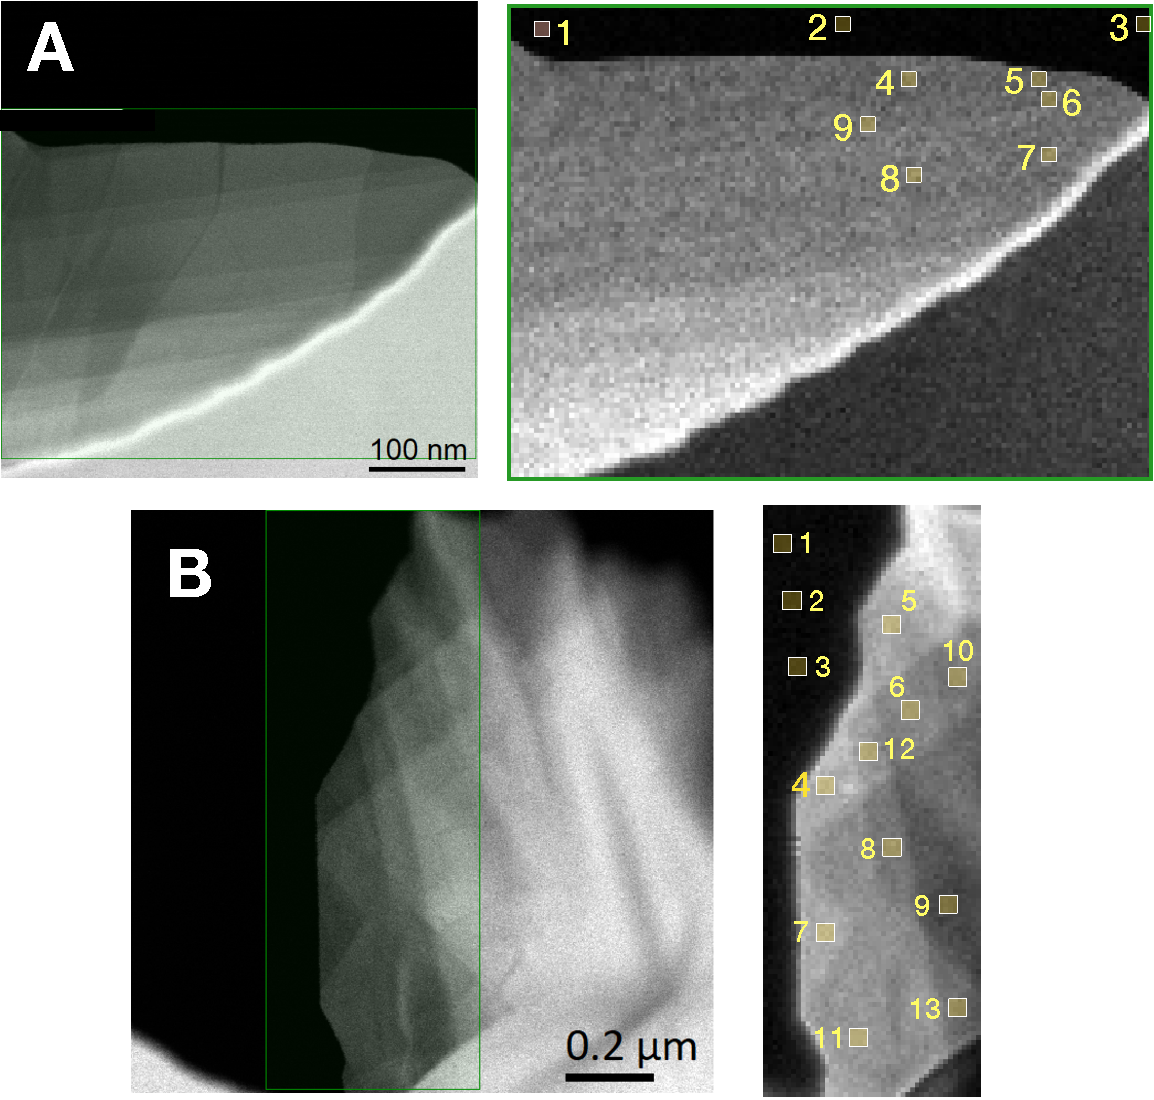
\includegraphics[width=0.87\linewidth]{plots/Spectra_location.pdf}
  \caption{Low-magnification TEM images (left) and the corresponding
    spectral images (right panels) of two different regions of
    the WS$_2$ nanoflowers, denoted as sample A and sample B respectively.
    %
    The spectral images have been recorded in the region marked by a green square
    in the corresponding TEM images.
    %
    We indicate the locations where representative
    EEL spectra have been selected. 
    %
    In the left panel of sample B, the difference in contrast is correlated to the material
    thickness, with higher contrast corresponding to thinner regions of the nanostructure.
    %
    The morphological differences between the two samples are discussed in the text.
  }
\label{fig:ws2positions}
\end{centering}
\end{figure}
%%%%%%%%%%%%%%%%%%%%%%%%%%%%%%%%%%%%%%%%%%%%%%%%%%%%%%%%%%%%%%%%%%%%%%%%%%

In Table~\ref{table:sampledata} we collect the most relevant properties of the spectra collected
in the locations indicated in Fig.~\ref{fig:ws2positions} using the same format as
in Table~\ref{table:vacuumdata}.
%
Note that since the of spectra from samples A and B
have been acquired with different microscopes, features of the ZLP
such as the FWHM are expected to be different.
%
From this table one can observe how the ZLP for the spectra acquired on sample A exhibit
a FWHM about three times larger as compared to those of sample B.
%
This difference in resolution can be understood from the fact that the EELS spectra from sample B, unlike those
from sample A, were recorded with a TEM equipped with a monochromator.

%%%%%%%%%%%%%%%%%%%%%%%%%%%%%%%%%%%%%%%%%%%%%%%%%%%%%%%%%%%%%%%%%%%%%%%%%%%%%%%%%%%%%%%%%%%%%
%%%%%%%%%%%%%%%%%%%%%%%%%%%%%%%%%%%%%%%%%%%%%%%%%%%%%%%%%%%%%%%%%%%%%%%%%%%%%%%%%%%%%%%%%%%%%
\begin{table}[t]
  \begin{center}
            \renewcommand{\arraystretch}{1.50}
  \begin{tabular}{@{}ccccccccc}
\br
Set & $t_{\rm exp}$ {(}ms{)} & $E_{\rm b}$ {(}keV{)} & $N_{\rm sp}$ & $N_{\rm dat}$ & $\Delta E_{\rm min}$~(eV)  & $\Delta E_{\rm max}$~(eV)  & FWHM~(eV)  \\ 
\mr
A        &       1       &        60         &   6      &    1918    &     -4.1       & 45.5 & $ 0.47\pm0.01$  \\
B        &       190       &        60       &   10     &    2000    &     -0.9        & 9.1   & $ 0.16\pm0.01$ \\
\br
  \end{tabular}
    \end{center}
  \caption{\small Same as Table~\ref{table:vacuumdata} now for the EEL spectra taken on specimens A and B.
    %
    Note that the location on the WS$_2$ nanoflowers where each spectra has been recorded
    was indicated in Fig.~\ref{fig:ws2positions}.
  }
   \label{table:sampledata}
\end{table}
%%%%%%%%%%%%%%%%%%%%%%%%%%%%%%%%%%%%%%%%%%%%%%%%%%%%%%%%%%%%%%%%%%%%%%%%%%%%%%%%%%%%%%%%%%%%%%%%%5
%%%%%%%%%%%%%%%%%%%%%%%%%%%%%%%%%%%%%%%%%%%%%%%%%%%%%%%%%%%%%%%%%%%%%%%%%%%%%%%%%%%%%%%%%%%%%

In the following we will present the results for representative spectra
corresponding to each of the two samples.
%
The full set of spectra is available together with {\tt EELSfitter},
the code used to produce the results of this analysis,
whose installation
and usage instructions are presented in Appendix~\ref{sec:installation}.

\subsection{Subtraction procedure}

In Table~\ref{table:sampledata_summary} we collect
the mean value and uncertainty of the first local minimum, $\Delta E|_{\rm min}$.
averaged over the spectra corresponding to samples A and B from
Fig.~\ref{fig:ws2positions}.
%
The location of the first minimum is relatively stable
among all the spectra belonging to a given set.
%
This indicates that the onset of the inelastic contributions $I_{\rm inel}$ does
not change significantly as we move to different regions of the sample.
%
We also indicate
the corresponding values of the hyper-parameters
$\Delta E_{\rm I}$ and $\Delta E_{\rm II}$ defined in Fig.~\ref{fig:EELS_toy}.
%
Recall that only
the data points with $\Delta E \le \Delta E_{\rm I}$ is used for the training
of the neural network model.
%
For $\Delta E \ge \Delta E_{\rm II}$ instead, the training set includes only the pseudo-data
that implements the $I_{\rm ZLP}(\Delta E)\to 0$ constraint.
 %
The values for $\Delta E_{\rm II}$ were determined from the vacuum recorded spectra
following the same procedure as explained 
in Sect.~\ref{sec:results_vacuum}.
%
We note that the values of $\Delta E_{\rm II}$ for this part are significantly higher than
the ones found in Fig.~\ref{fig:intensityratio}. This could be ascribed to the fact that 
the vacuum spectra from sample A and B are recorded in proximity to a sample, and therefore
effects from the sample are still present, although at a reduced rate.
 %
The model training is performed for a range of $\Delta E_{\rm I}$ values
subject to the condition that $\Delta E_{\rm I} \le \Delta E_{\rm min}$.

%%%%%%%%%%%%%%%%%%%%%%%%%%%%%%%%%%%%%%%%%%%%%%%%%%%%%%%%%%%%%%%%%%%%%%%%%%%%%%%%%%%%%%%%%%%%%
%%%%%%%%%%%%%%%%%%%%%%%%%%%%%%%%%%%%%%%%%%%%%%%%%%%%%%%%%%%%%%%%%%%%%%%%%%%%%%%%%%%%%%%%%%%%%
\begin{table}[t]
  \begin{center}
            \renewcommand{\arraystretch}{1.50}
  \begin{tabular}{@{}ccccccccc}
\br
Set & $\Delta E|_{\rm min}$~(eV)  &  $\Delta E_{\rm I}$~(eV)  &  $\Delta E_{\rm II}$~(eV)   \\
\mr
A        &    $2.70\pm0.06$               &          1.8        &      12         \\
B        &    $1.80\pm0.04$               &          1.4        &      6        \\
\br
  \end{tabular}
    \end{center}
  \caption{\small The mean value and uncertainty of the first local minima, $\Delta E|_{\rm min}$,
    averaged over the spectra corresponding to samples A and B from
    Fig.~\ref{fig:ws2positions}.
    %
    We also indicate
     the corresponding values of the hyper-parameters
     $\Delta E_{\rm I}$ and $\Delta E_{\rm II}$ defined in Fig.~\ref{fig:EELS_toy} used for the training
     of the neural network model.
    %
  }
   \label{table:sampledata_summary}
\end{table}
%%%%%%%%%%%%%%%%%%%%%%%%%%%%%%%%%%%%%%%%%%%%%%%%%%%%%%%%%%%%%%%%%%%%%%%%%%%%%%%%%%%%%%%%%%%%%%%%%5
%%%%%%%%%%%%%%%%%%%%%%%%%%%%%%%%%%%%%%%%%%%%%%%%%%%%%%%%%%%%%%%%%%%%%%%%%%%%%%%%%%%%%%%%%%%%%

The optimal values of $\Delta E_{\rm I}$ listed in Table~\ref{table:sampledata_summary} are
determined as follows.
%
We evaluate the ratio
between the derivative of the intensity distribution acquired on the specimen over the
same quantity recorded in vacuum,
\be
\label{eq:rder}
\mathcal{R}^{(j)}_{\rm der}(\Delta E) \equiv
\la
\frac{
  dI_{\rm EEL}^{({\rm exp})(j)}(\Delta E)/ d\Delta E
}{
  dI_{\rm EEL}^{({\rm exp})(j')}(\Delta E) /d\Delta E
} \ra_{N_{\rm sp}' } \, ,
\ee
where $j'$ labels one of the $N_{\rm sp}'$ vacuum spectra and the average is taken
over all available values of $j'$.
%
This ratio allows to identify a suitable value of $\Delta E_{I}$ by establishing
for which energy losses the shape (rather than the absolute value) of the intensity distributions 
recorded on the specimen starts to differ significantly from their vacuum counterparts.
%
A sensible choice of $\Delta E_{\rm I}$ could for instance be given by
$\mathcal{R}_{\rm der}(\Delta E_{\rm I}) \simeq 0.8$, for which derivatives differ
at the 20\% level.
%
Note also that the leftmost value of the energy loss satisfying
$\mathcal{R}_{\rm der}(\Delta E)=0$ in Eq.~(\ref{eq:rder}) corresponds to the position of the first
local minimum of the spectrum.

The end result of the  neural network training is
 a set of $N_{\rm rep}=500$ replicas
  parametrising the ZLP, $I_{\rm ZLP}^{({\rm mod})(k)}(\Delta E)$.
 %
 Taking into account that we have $N_{\rm sp}$ individual spectra in each sample,  the ZLP
 subtraction is performed individually
 for each Monte Carlo replica,
 \be
 \label{eq:subtractedModelPrediction}
 I_{\rm inel}^{({\rm exp})(j,k)}(\Delta E) \equiv I_{\rm EELS}^{({\rm exp})(j)}(\Delta E) - I_{\rm ZLP}^{({\rm mod})(k)}(\Delta E)\, ,
 \quad \forall~N_{\rm rep} \, ,\quad j=1,\ldots,N_{\rm sp} \, ,
 \ee
 from which statistical estimators can be evaluated as usual.
 %
 For instance, the mean value for our model prediction for the $j$-th spectrum
 can be evaluated by averaging over the set of replicas,
 \be
 \la  I_{\rm inel}^{({\rm exp})({\rm (exp)}j)}\ra (\Delta E)
 = \frac{1}{N_{\rm rep}} \sum_{k=1}^{N_{\rm rep}}  I_{\rm inel}^{({\rm mod})(j,k)}(\Delta E) \, ,
 \quad j=1,\ldots,N_{\rm sp} \, ,
 \ee
 and likewise for the corresponding uncertainties or correlations.
%
 For large values of $\Delta E$
 the model prediction reduces to the original spectra, since in that region
 the ZLP contribution vanishes,
 \be
 I_{\rm inel}^{({\rm exp})(j,k)}(\Delta E \gg \Delta E_{\rm I}) \to  I_{\rm EE}^{{\rm (exp)}(j)}(\Delta E) \, ,\quad
 \forall~j,k \, .
 \ee
 
 For very small values of the energy loss, the contribution to the total
 spectra from inelastic scatterings is negligible
 and thus the subtracted model prediction Eq.~(\ref{eq:subtractedModelPrediction}) should
 vanish.
 %
 However, this will not be the case in practice since the neural-net model is trained on
 the $N_{\rm sp}$ ensemble of spectra, rather that just on individual ones, and thus the expected
 $\Delta E \to 0$ behaviour will only be achieved within uncertainties rather than at the level of
 central values.
 %
 To achieve the desired $\Delta E \to 0$ limit, we apply a matching procedure
 as follows.
 %
 We introduce another hyper-parameter, $\Delta E_0 < \Delta E_1$, such that
 one has for the $k$-th ZLP replica associated to the $j$-th spectrum the following
 behaviour:
 \bea
 \nonumber
 I_{\rm ZLP}^{({\rm mod})(j,k)}(\Delta E) &=& I_{\rm EELS}^{({\rm exp})(j)}(\Delta E) \, ,\quad \Delta E < \Delta E_0  \, ,\\
 I_{\rm ZLP}^{({\rm mod})(j,k)}(\Delta E) &=& I_{\rm EELS}^{{\rm (exp)}(j)} + \lp \xi_1^{(n_l)(k)}(\Delta E) -
 I_{\rm EELS}^{{\rm (exp)}(j)}(\Delta E)\rp  \times \mathcal{F} \, , \nonumber \quad 
 \Delta E_0 < \Delta E \le \Delta E_1 \, ,\\
 &&\mathcal{F} = \exp\lp -\frac{\lp \Delta E - \Delta E_1 \rp^2 }{\lp \Delta E_0 - \Delta E_1 \rp^2 \delta^2} \rp  \, , \label{eq:matching} \\
 I_{\rm ZLP}^{({\rm mod})(j,k)}(\Delta E) &=& \xi_1^{(n_l)(k)}(\Delta E) \, , \quad \Delta E > \Delta E_1 \nonumber \, ,
 \eea
 where $\xi_1^{(n_l)(k)}$ indicates the output of the $k$-th neural network that parametrises
 the ZLP and $\delta$ is a dimensionless tunable parameter.
 %
 In Eq.~(\ref{eq:matching}), $\mathcal{F}(\Delta E)$ represents a matching factor
 that ensures that the ZLP model prediction smoothly interpolates
 between $\Delta E=\Delta E_0$ (where $\mathcal{F}\ll 1$ and the original spectrum should
 be reproduced) and $\Delta E=\Delta E_1$
 (where $\mathcal{F}=1$ leaving the neural network output unaffected).
 %
 Here we adopt $\Delta E_0 = \Delta E_1 -0.5\,{\rm eV}$,  having verified
 that results are fairly independent of this choice.
 %
 Taking into account the matching procedure, we can slightly modify Eq.~(\ref{eq:subtractedModelPrediction})
 to 
 \be
 \label{eq:subtractedModelPrediction2}
 I_{\rm inel}^{({\rm mod})(j,k)}(\Delta E) \equiv I_{\rm EELS}^{({\rm exp})(j)}(\Delta E) - I_{\rm ZLP}^{({\rm mod})(j,k)}(\Delta E)\, ,
 \quad \forall~N_{\rm rep} \, ,\quad j=1,\ldots,N_{\rm sp} \, .
 \ee

 The ensemble of ZLP-subtracted spectra $\{I_{\rm inel}^{({\rm mod})(j,k)} \} $
 can then be used to estimate the bandgap of the specimen in the region where
 they were acquired.
 %
 Different approaches  have been put forward to estimate the value of the bandgap from 
subtracted EEL spectra, \textit{e.g.} by means of the inflection point of the rising intensity or
a linear fit to the maximum positive slope~\cite{Schamm:2003}.
%
Here we will adopt the approach of~\cite{Rafferty:2000} where the behaviour
of $I_{\rm inel}(\Delta E)$ in the onset region is modeled as
\begin{equation}
  \label{eq:I1}
    I_{\rm inel}(\Delta E) \simeq  A \lp \Delta E-E_{\rm BG} \rp^{b} \, , \quad \Delta E \ge E_{\rm BG} \, ,
\end{equation}
and vanishes for $E < E_{\rm BG}$, where both the bandgap value
$E_{\rm BG}$ as well as the parameters $A$ and $b$ are extracted from the fit.
%
The exponent $b$ is expected to be $b\simeq 1/2~(3/2)$ for a semiconductor material characterised
by a direct~(indirect) bandgap.
 %
 For each of the $N_{\rm sp}$ spectra and the $N_{\rm rep}$ replicas
 we fit to Eq.~(\ref{eq:subtractedModelPrediction2}) the model Eq.~(\ref{eq:I1})
 within a range taken to be
 $\lc \Delta E_{\rm I} - 0.5~{\rm eV}, \Delta E_{\rm I} + 0.7~{\rm eV}\rc$.
 %
 One ends up with $N_{\rm rep}$ values for
 the bandgap energy and fit exponent for each spectra,
 \be
 \Big \{ E_{\rm BG}^{(j,k)}, b^{(j,k)} \Big\} \, , \quad k=1,\ldots,N_{\rm rep} \, ,
 \quad j=1,\ldots,N_{\rm sp} \, ,
 \ee
 from which again one can readily evaluate their statistical estimators.
 %
 In the following, we will display the median and the 68\% confidence level intervals
 for these parameters to account for the fact that their distribution will be in general non-Gaussian.

 \subsection{Bandgap analysis}

We present first the results of the bandgap analysis of sample A,
taking location sp\#4 in Fig.~\ref{fig:ws2positions} as representative spectrum; compatible results
are found for the rest of locations.
%
As mentioned above, this region is characterised by a sizable thickness where
WS$_2$ is expected to behave as a bulk material.
%
The left panel of Fig.~\ref{fig:sp14_subtracted_spectrum} displays the original
and subtracted EEL spectrum
together with the predictions of the ZLP model, where
the bands indicate the 68\% confidence level uncertainties and the central value
is the median of the distribution.
%
The inset shows the result of the polynomial fits using Eq.~(\ref{eq:I1}) to the subtracted spectrum
together with the corresponding uncertainty bands.

%%%%%%%%%%%%%%%%%%%%%%%%%%%%%%%%%%%%%%%%%%%%%%%%%%%%%%%%%%%%%%%%%%%%%%%
\begin{figure}[t]
\begin{centering}
  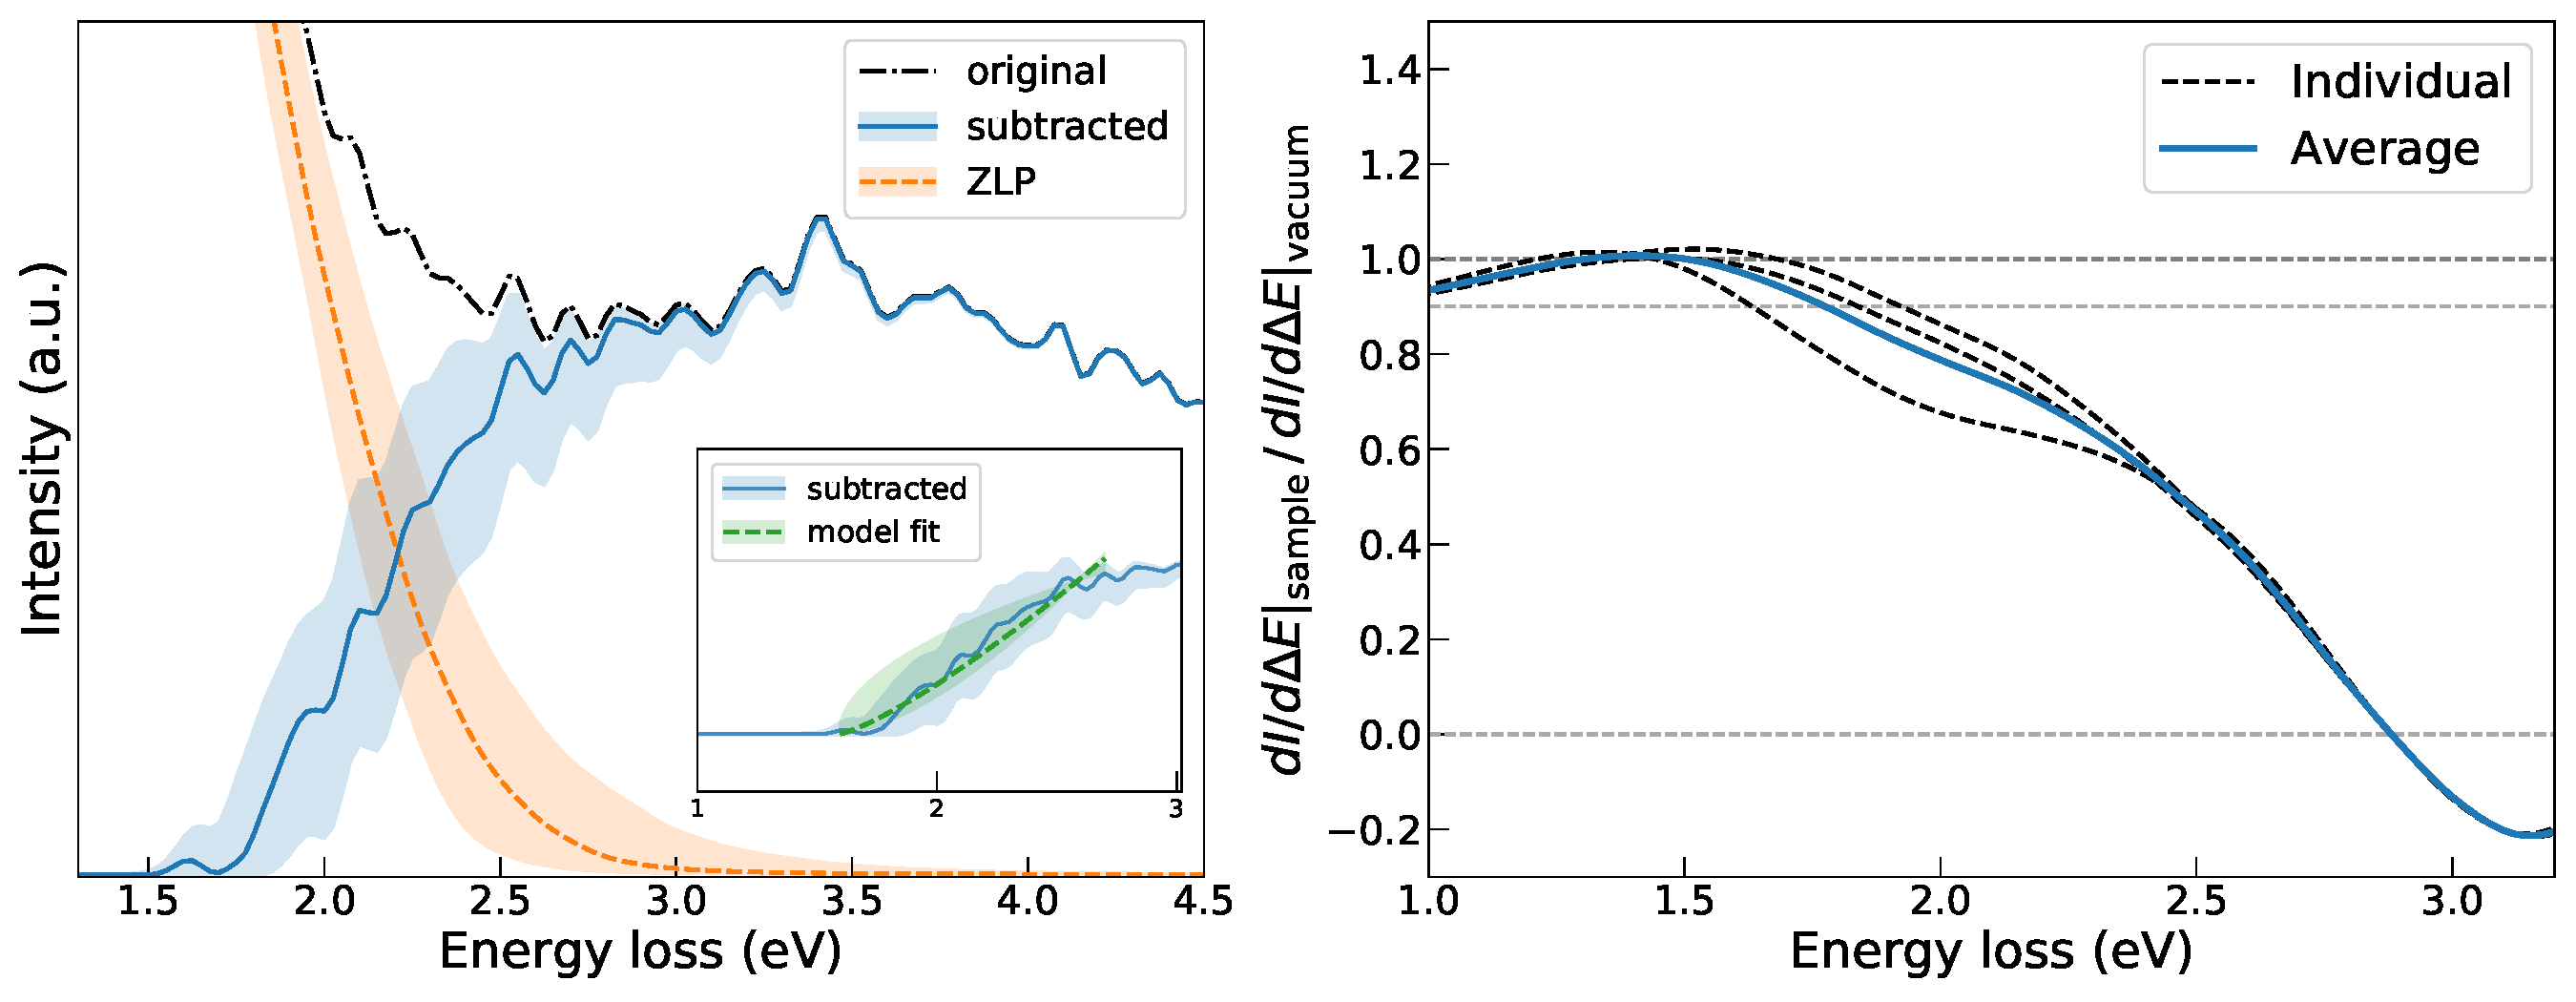
\includegraphics[width=0.99\linewidth]{plots/SubtractedEELS_plot_sp14.pdf}
   \caption{Left: the original
     and subtracted EEL spectrum corresponding to location \#4 of sample A in Fig.~\ref{fig:ws2positions},
     together with the predictions of the ZLP model, where
     the bands indicate the 68\% confidence level uncertainties.
     %
     The inset displays the result of fitting Eq.~(\ref{eq:I1}) to the onset
     region of the subtracted spectrum.
     %
     Right: the average ratio of the derivative of the intensity
     distribution in sp4 over its vacuum counterpart, Eq.~(\ref{eq:rder})
  }
\label{fig:sp14_subtracted_spectrum}
\end{centering}
\end{figure}
%%%%%%%%%%%%%%%%%%%%%%%%%%%%%%%%%%%%%%%%%%%%%%%%%%%%%%%%%%%%%%%%%%%%%%%%%%

One can observe how the ZLP model uncertainties are small at low $\Delta E$
(due to the matching condition) and large $\Delta E$ (where the ZLP vanishes),
but become significant in the intermediate region where the contributions
from $I_{\rm ZLP}$ and $I_{\rm inel}$ become comparable.
%
It is worth emphasizing that these (unavoidable) uncertainties are neglected in most
ZLP subtraction methods.
%
The validity of our choice for the hyperparameter $\Delta E_{\rm I}$ (Table~\ref{table:sampledata_summary})
can be verified {\it a posteriori} by evaluating the ratio
\be
\mathcal{R}^{(j)}_{\rm abs}\lp \Delta E_{\rm I}\rp \equiv 
\la I_{\rm ZLP}^{({\rm mod})(j)}\ra_{\rm rep} \Big/I_{\rm EEL}^{({\rm exp})(j)} \Big|_{\Delta E = \Delta E_{\rm I}} \, ,
\ee
which in this case turns out to be $\mathcal{R}_{\rm abs} = 0.98$.
%
It is indeed important to verify that $\mathcal{R}_{\rm abs}\lp \Delta E_1\rp$ is not too far from unity,
indicating that the training dataset has not been contaminated by the inelastic contributions.

The average ratio of the derivative of the intensity
distribution in spectrum 4 over its vacuum counterpart, Eq.~(\ref{eq:rder}), is shown
in the right panel of  Fig.~\ref{fig:sp14_subtracted_spectrum}. 
%
By requiring that $\mathcal{R}^{(j)}_{\rm der}(\Delta E_{\rm I})\simeq 0.9$ we obtain
the value $\Delta E_{\rm I}=1.8$ eV used as baseline the analysis.
%
It should be noted that this choice is not unique, for example requiring
$\mathcal{R}^{(j)}_{\rm der}(\Delta E_{\rm I})\simeq 0.8$ instead would have led
to $\Delta E_{\rm I}=2.0$ eV.
%
It is therefore important to asses the stability of our results as the hyper-parameter $\Delta E_{\rm I}$
is varied around its optimal value.

With this motivation, in Fig.~\ref{fig:bvalues_sampleA} we display the
values of the exponent $b$
and the bandgap energy $E_{\rm BG}$ 
obtained from the same subtracted spectrum as that shown in
Fig.~\ref{fig:sp14_subtracted_spectrum} for variations of $\Delta E_{\rm I}$ 
around its optimal value (1.8 eV, indicated by the horizontal dashed line) by an amount
of $\pm 0.2$ eV.
%
Here the central value and the error band for each value of $\Delta E_I$ is evaluated
as the median and the 68\% CL interval over the $N_{\rm rep}=500$ Monte Carlo replicas.
%
We observe that the model predictions for both $b$ and $E_{\rm BG}$ are stable with respect
to variations of $\Delta E_I$, with any shift in the central value contained within the
uncertainty bands.
%
We can therefore conclude that our approach is robust with respect to the choice of its
hyper-parameters.

%%%%%%%%%%%%%%%%%%%%%%%%%%%%%%%%%%%%%%%%%%%%%%%%%%%%%%%%%%
\begin{figure}[t]
\begin{centering}
  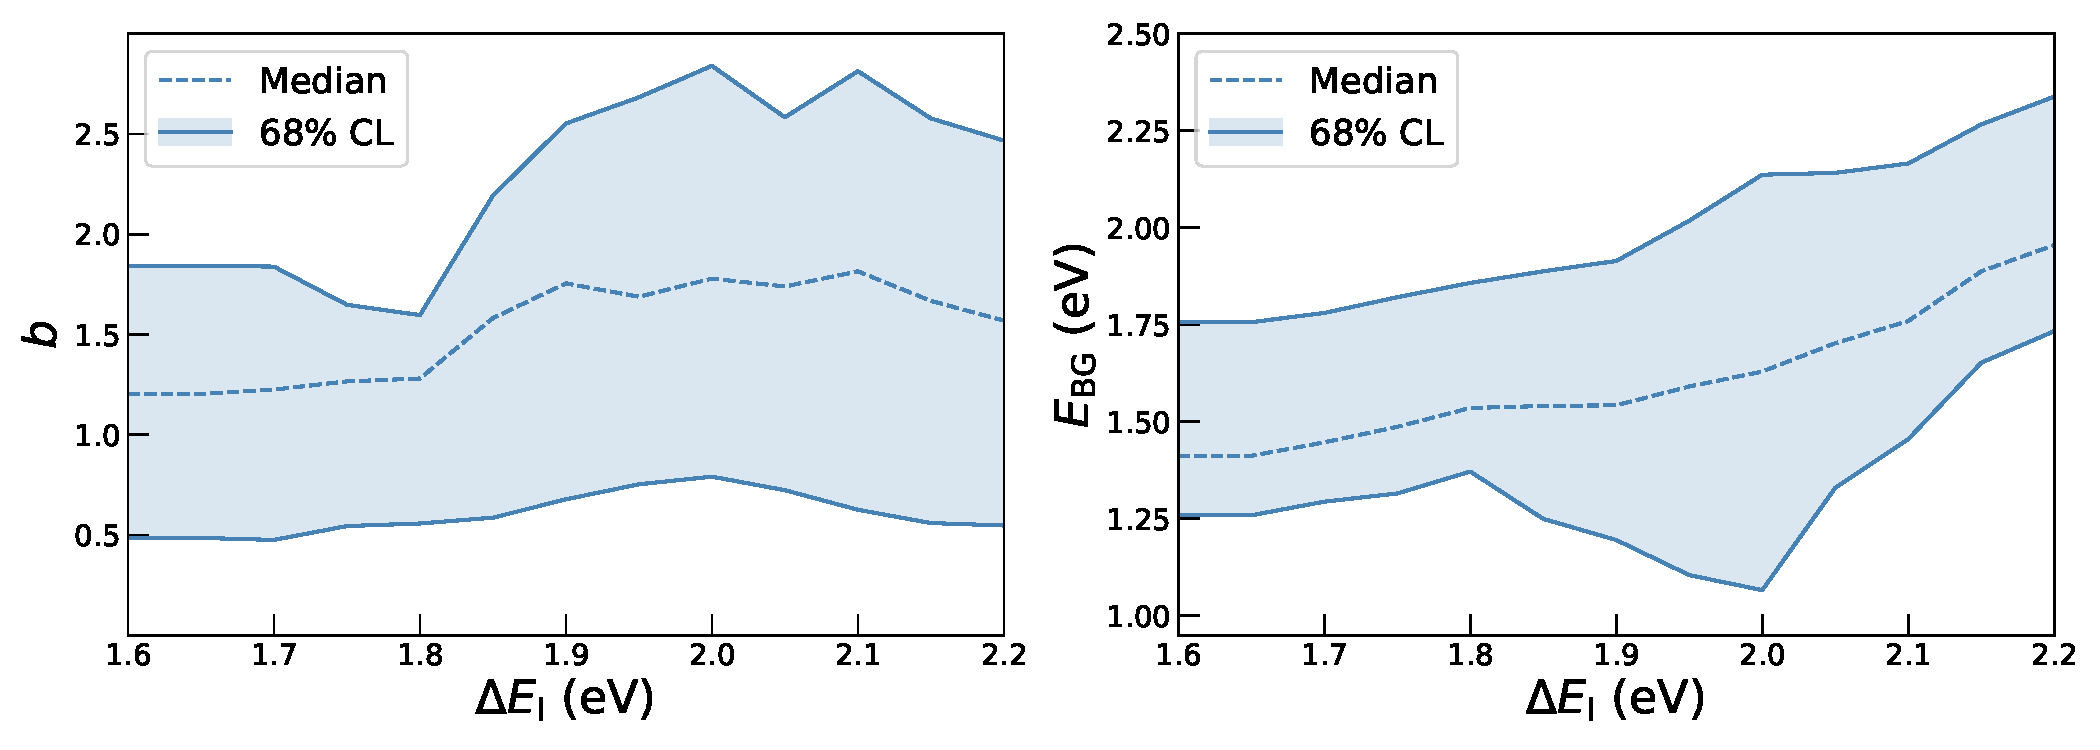
\includegraphics[width=0.99\linewidth]{plots/Stability_plots_sp14.pdf} 
  \caption{\small The values of the exponent $b$ (left)
    and the bandgap energy $E_{\rm BG}$ (right panel) from the model Eq.~(\ref{eq:I1})
    obtained from the subtracted spectrum sp14 as $\Delta E_{\rm I}$ is varied by $\pm 0.2$ eV
    around its optimal value, indicated by the horizontal dashed line.
  }
\label{fig:bvalues_sampleA}
\end{centering}
\end{figure}
%%%%%%%%%%%%%%%%%%%%%%%%%%%%%%%%%%%%%%%%%%%%%%%%%%%%%%%%%%%%%

The final values for $E_{\rm BG}$ and $b$ obtained in the analysis of this specific spectrum are
\be
E_{\rm BG} = 1.6_{-0.2}^{+0.3}\,{\rm eV} \, ,\quad b= 1.3_{-0.7}^{+0.3} \, .
\ee
We thus find that for this specific region of the WS$_2$ nanoflowers
the model fit to the subtracted EEL spectrum exhibits a clear preference
for an indirect bandgap (where $b\simeq 1.5$), though a direct one ($b\simeq 0.5$)
cannot be excluded within uncertainties.
%
This result is consistent with the theoretical expectations of the local
electronic properties of bulk WS$_2$.
%
Further, the value of $E_{\rm BG}$ is consistent with previous determinations
in the same material at the bulk level, such as those collected in Table~\ref{table:bgvalues}.
%
Consistent results are obtained for other locations of Fig.~\ref{fig:ws2positions}
where spectra have been recorded.
%
To the best of our knowledge
these results represent the first EELS bandgap analysis of WS$_2$ nanostructures
whose crystalline structure is based on mixed 2H/3R polytypes.

\subsection{Mapping excitonic transitions in the low-loss region}

Concerning the EEL spectra recorded in sample B (bottom panels
in  Fig.~\ref{fig:ws2positions}), the same criterion
for the derivative ratio Eq.~(\ref{eq:rder}) indicates now that $\Delta E_I\simeq 1.4$ eV,
a somewhat lower value as the corresponding one obtained for sample A.
%
The left panel of Fig.~\ref{fig:SubtractedEELS_plot_sp4} displays
the original
and subtracted EEL spectra corresponding to location sp4 of sample B in Fig.~\ref{fig:ws2positions},
together with the predictions of the ZLP model.
%
As in Fig.~\ref{fig:sp14_subtracted_spectrum}, the bands indicate the 68\% confidence level uncertainties.
%
The main difference with respect to the spectra recorded in sample A is the appearance of well-defined
features (peaks) in the subtracted spectrum already at very small values of $\Delta E$.
%
In particular, we observes two marked peaks at $\Delta E\simeq 1.5$ and 2.0 eV and a
softer one near $\Delta E=1.7$ eV.

%%%%%%%%%%%%%%%%%%%%%%%%%%%%%%%%%%%%%%%%%%%%%%%%%%%%%%%%%%%%%%%%%%%%%%%
\begin{figure}[t]
\begin{centering}
  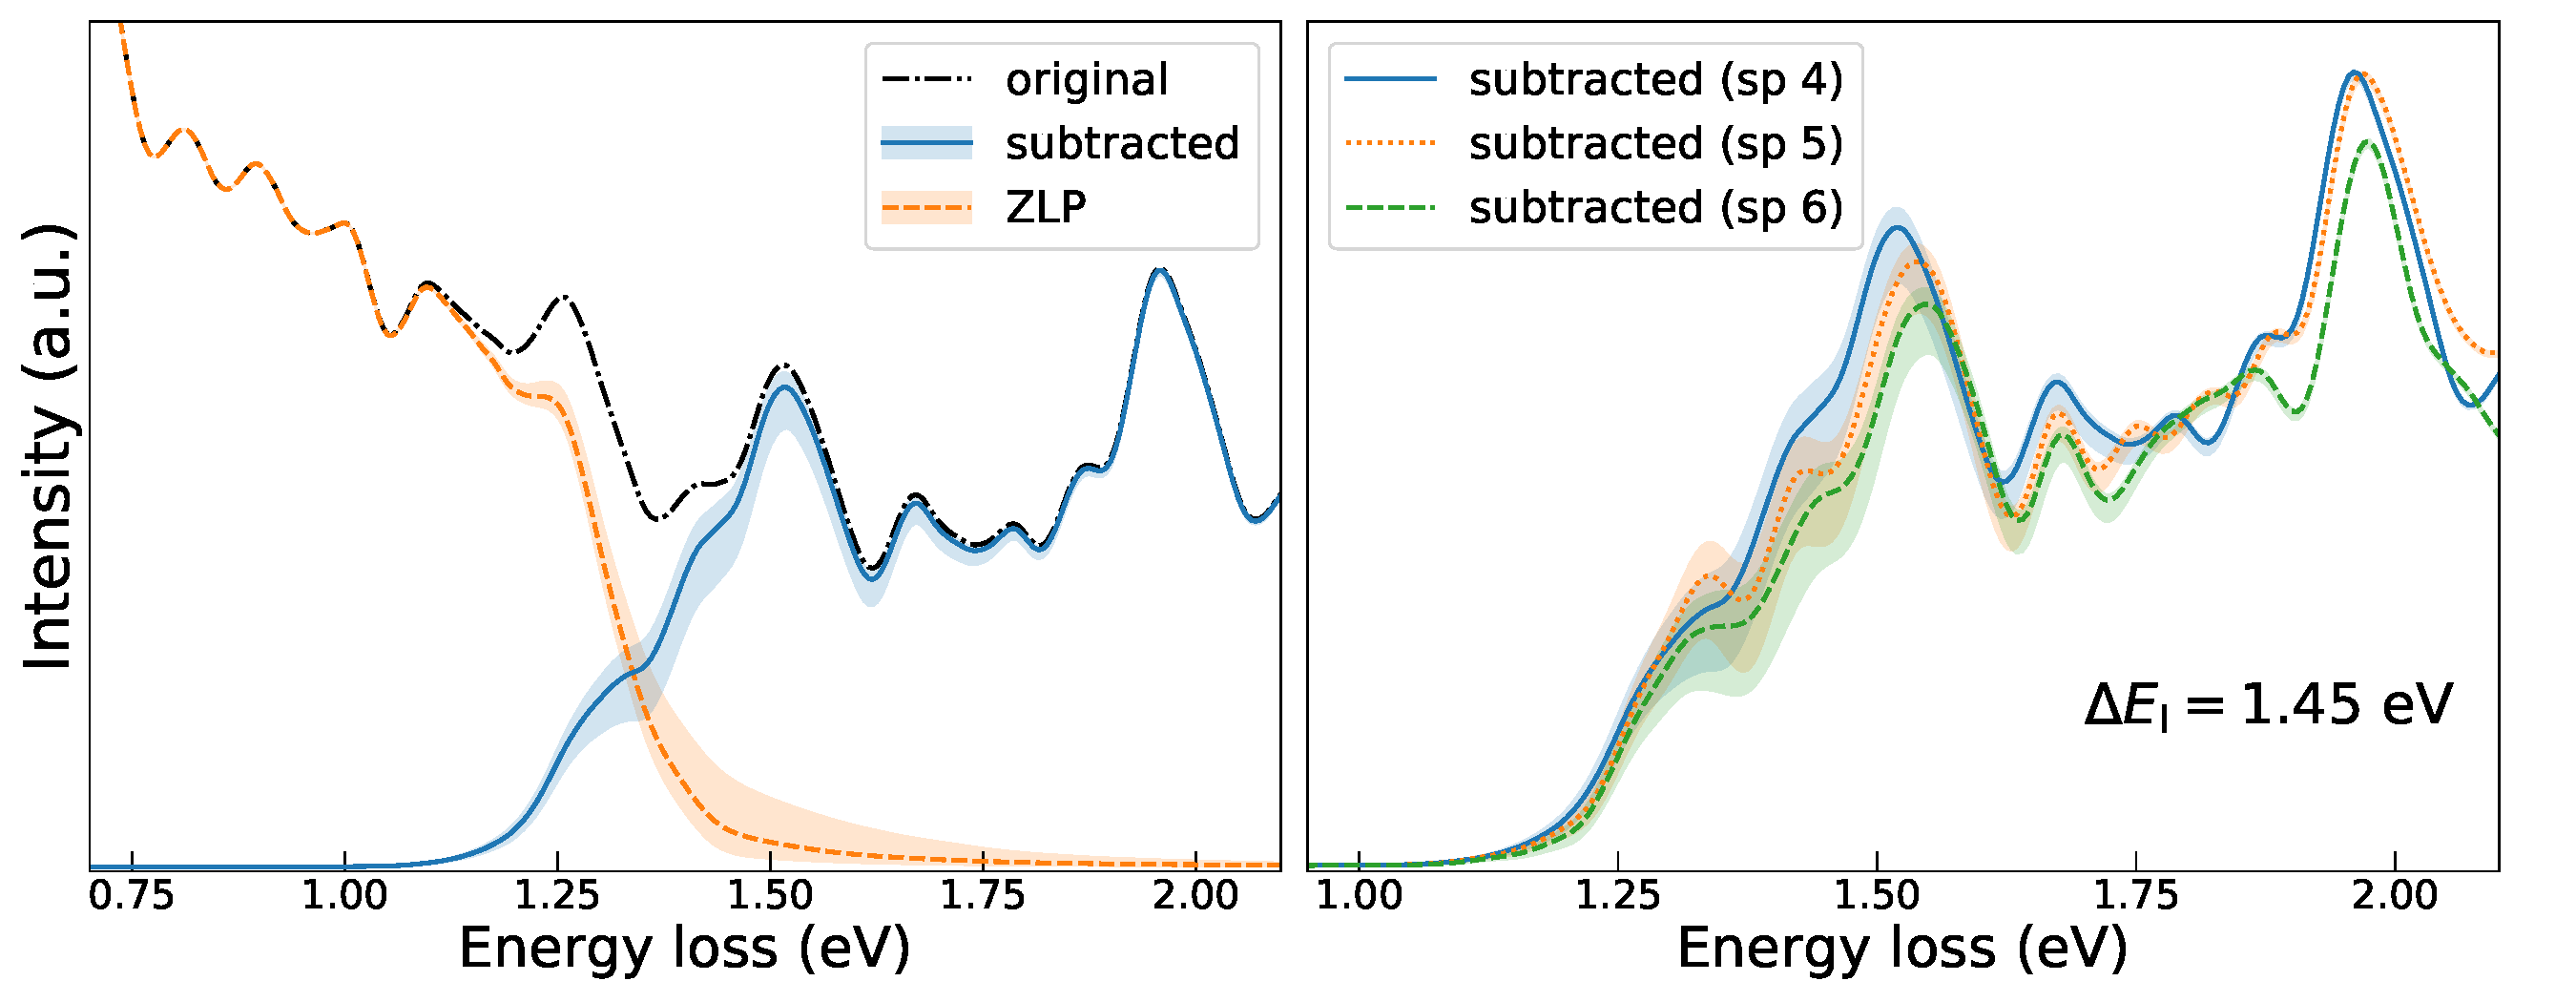
\includegraphics[width=0.99\linewidth]{plots/subtractedEELS_plot_sampleB_sp4.pdf}
  \caption{Left: the original
     and subtracted EEL spectra corresponding to location sp4 of sample B in Fig.~\ref{fig:ws2positions},
     together with the predictions of the ZLP model.
     %
     The bands indicate the 68\% confidence level uncertainties.
     %
     Right: comparison of the ZLP-subtracted spectra from locations sp4, sp5, and sp6 in sample B
     together with the corresponding model uncertainties.
    %
     Note how the features of the subtracted spectra, such as the peaks as $\Delta E\simeq 1.5$,
    1.7 and 2.0 are eV, are common across the three locations.
  }
\label{fig:SubtractedEELS_plot_sp4}
\end{centering}
\end{figure}
%%%%%%%%%%%%%%%%%%%%%%%%%%%%%%%%%%%%%%%%%%%%%%%%%%%%%%%%%%%%%%%%%%%%%%%%%%

There are two dominant factors that explain the differences in the EEL spectra recorded
in samples A and B.
%
The first one is the former is much thicker (bulk material) while the latter corresponds
to thin, overlapping petals whose thickness can be as small as a few monolayers.
%
The second is that the measurements taken in sample A used a TEM without monochromator,
while those of sample B benefited from a monochromator and thus achieves a superior
spectral resolution (average FWHM being 16 meV, to be compared with the 470 meV of sample A, see
Table~\ref{table:sampledata}).
%
Therefore, the combination of structural and morpholical differences in the specimen together
with the different operation conditions of the TEM account for most of the differences
between the two set of spectra.


bandgap not suitable


statistical fluctuations

Fig.~\ref{fig:subtracted_spectra_comp} displays the
the ZLP-subtracted spectra from sample B corresponding to locations sp4, sp5, and sp6
    from Fig.~\ref{fig:ws2positions} together with the corresponding model uncertainties.
    %
    Results are shown for two values of the hyperparameter $\Delta E_{\rm I}$,
    1.45 eV (left) and 1.55 eV (right panel).
    %
    Note how features of the subtracted spectra such as the peaks as $\Delta E\simeq 1.5$,
    1.7 and 2.0 are common across the three spectra, demonstrating that there
    are genuine physical features of the ultra-low-loss region rather than statistical
    fluctuations.
    %
The research on fundamental optical properties of TMDs has led to the discovery of different 
types of exciton transitions in the ultra-low-loss region of WS$_2$ nanostructures. 
%
The origin of these peaks can be attributed to the formation of an electron-hole pair mitigated
by the dielectric screening from the surrounding lattice~\cite{Hanbicki:2016}.
%
In reduced dimensions as in single layers of TMDs, exciton peaks arise with binding energies
up to ten times larger than for bulk structures.
%
In the optical spectra of TMDs, two strongly pronounced resonances denoted by A and B
excitons are often observed, appearing at binding energies of 300-500 meV below the true band gap~\cite{Karivaj:2019}.
%
This is in accordance with the features observed in Fig.~\ref{fig:subtracted_spectra_comp} at 
$\Delta E\simeq 1.5$ and 1.7 eV, which is exactly 300-500 meV below the true bandgap value
expected for 2D structures of WS$_2$. 
%
The presence of these low loss features makes the bandgap analysis on this sample 
non-trivial, since one can only fit Eq.~(\ref{eq:I1}) to the onset region of the 
bandgap excitation. 
%
Nevertheless, the ZLP-subtracted spectra in Fig.~\ref{fig:subtracted_spectra_comp} show that
we have been able to cleanly resolve exciton features down to 1.5 eV within appropriate
uncertainty.


